\chapter{Solution Idea} \label{chap:solutionideas}

This section presents our plan for obtaining the objectives discussed in the previous section. 
In our approach, we propose a Model-based Data-driven development approach involving a six-step solution:
\begin{itemize}
	\item \texttt{UI Prototyping} using the drag and drop approach.
	\item \texttt{Modelling} these prototypes.
	\item Creating \texttt{Experiments} from the models and assigning them to the users. 
	\item \texttt{A/B testing}.
	\item \texttt{Quantitative analysis}. 
	\item \texttt{Qualitative analysis}. 
\end{itemize}
As per the LEAN development Model (see Figure \ref{intro:fig:lean}), the \texttt{UI Prototyping} and the \texttt{Modelling} falls under the \texttt{Ideation} phase, the \texttt{Experiments} and \texttt{A/B Testing} which falls under \texttt{Coding} phase measure the data, and finally the \texttt{Qualitative} and \texttt{Quantitative} analysis which falls under \texttt{Data} phase learn and tune our models.

Let us understand the solution approach with the help of an example \textbf{``A video streaming service''} called \texttt{VideoStreamer (VS)}.
As shown in figure \ref{solutionideas:fig:stakeholders}, this company has different stakeholders e.g., users, developers, product owners, etc.
\begin{figure}
    \centering
    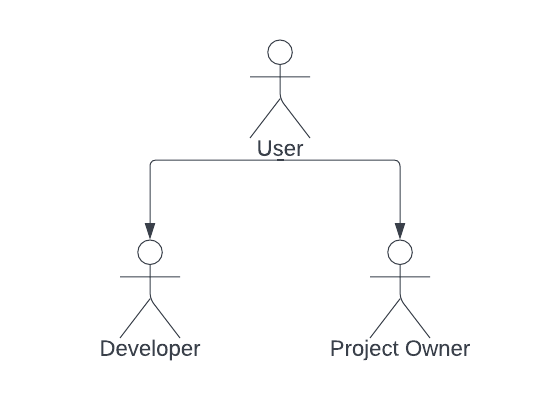
\includegraphics[scale=0.36]{images/solution-ideas/Stakeholder.png}
    \caption{Different Stakeholders in the Company VS}
    \label{solutionideas:fig:stakeholders}
\end{figure}
Usually, the developers are responsible for developing various features required for the company. 
But, the problem is, in the beginning, knowing which design fits better for a UI is impossible. 
Therefore, we need to perform experiments on the UI using A/B testing.
This approach has become very popular among developers. 
So, the developers develop different variants for experimenting with the UI and get feedback from the product owners. 
This feedback process wastes a lot of time, so our solution is to give freedom to the product owners and reduce the gap between the product owners and the developers by allowing the product owners to create the UI using UI prototyping.


\section{UI Prototyping} 

We plan to implement the UI prototyping in a low-code platform for our solution because it needs negligible installation, setup, training, and implementation work. 
The low-code platform enables rapid creation and deployment of business applications with the least amount of coding effort. 
We plan to set up a system for the product owner to modify the UI elements in a canvas-like structure in an application. 
For this, the product owners first create a canvas screen and input the name for that screen. 
As shown in the figure \ref{solutionideas:fig:uiprototyping}, they can add UI elements like buttons, input, select buttons, etc., on the canvas screen. 
We propose to use angular\footnote{Angular: \url{https://angular.io/}} for developing the application. 
Various UI elements are available for the drag and drop of the UI elements as shown in figure \ref{solutionideas:fig:uiprototyping} (right side).

\begin{figure}[h]
    \centering
    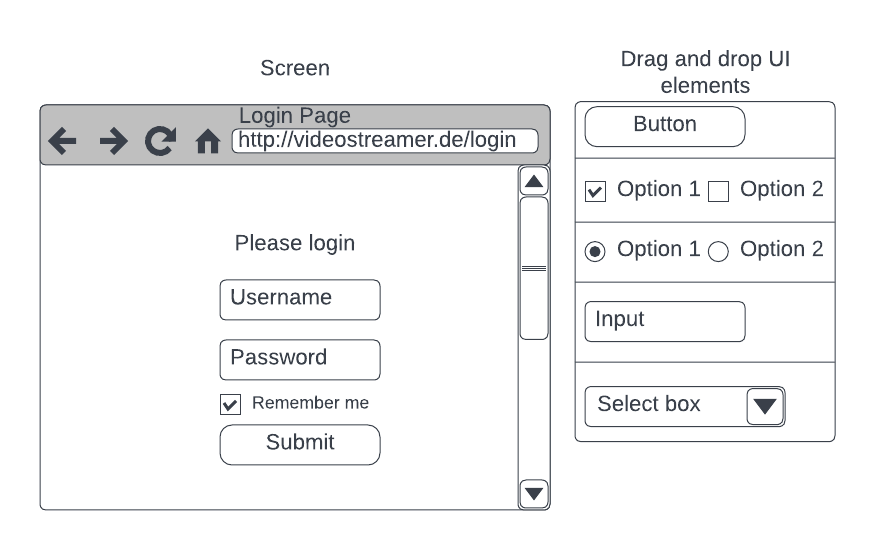
\includegraphics[scale=0.4]{images/solution-ideas/UIPrototyping.png}
    \caption{UI Prototyping using drag and drop od UI elements}
    \label{solutionideas:fig:uiprototyping}
\end{figure}

Once the UI screen is finalized, the product owner can move to the next screen by some logic (E.g., clicking on a button go to the next screen). 
This way, the product owner can design the entire application, having a semantic flow, using the canvas screen, and adjusting the UI elements. 

\section{Prototype Modelling}
\begin{figure}[ht]
	\centering
  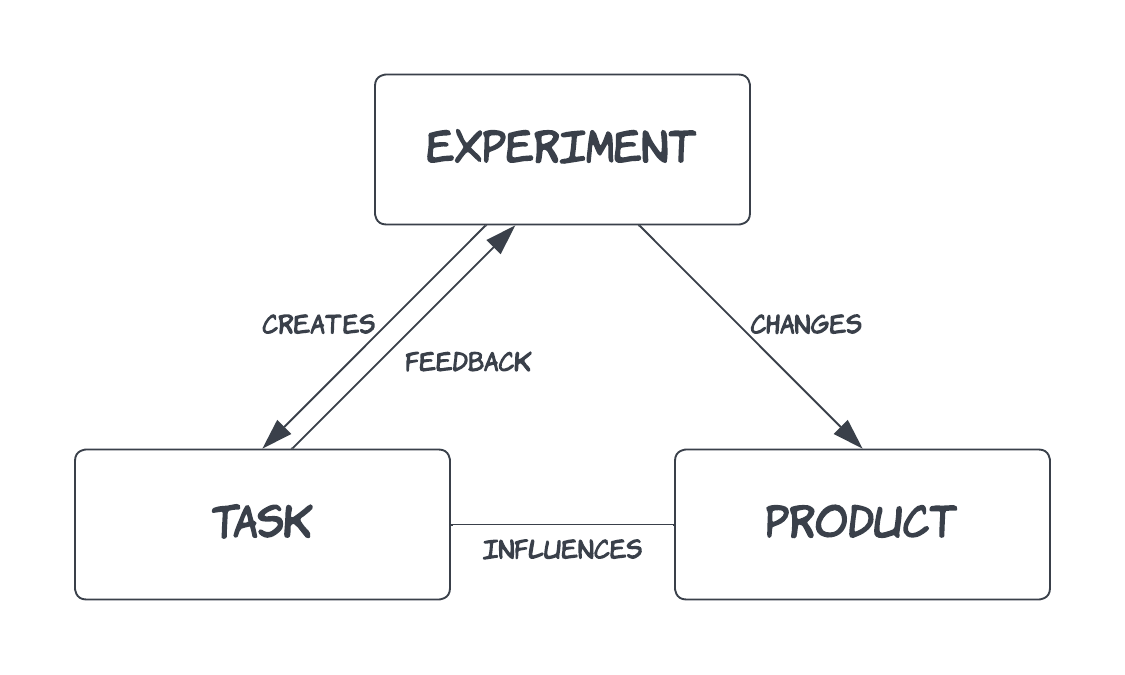
\includegraphics[width=0.7\textwidth]{images/solution-ideas/Triangle.png}
	\caption{Triangle of Experiment, Task and Product}
	\label{solutionideas:fig:triangle}
\end{figure}
 
In our application, we plan to convert the screens the product owner develops into models. 
To do that, we need a modeling language that fits our requirements. Based on our domain, we need models for \texttt{Experiments}, \texttt{Tasks} and \texttt{Products}.
\paragraph{Experiment:} In the \texttt{Experiment Model}, we store different properties of the UI elements along with the variant information.\\
E.g., from our \texttt{Videostreamer app}: If the experiment is on a \texttt{Button} element, our model should have information about the position of the button, the style of the button (storing the color, font, etc.), the title of the button, etc. All this information would be stored in the model as its properties or attributes.
Moreover, the model can obtain this information from the UI prototyping done by the product owner using drag and drop feature.
\paragraph{Product:} In the \texttt{Product Model}, we store information about the product and all its components as independent parts.\\
E.g., from our \texttt{Videostreamer app}: A video streamer would have different screens (see Fig \ref{solutionideas:fig:metamodel} right side), a Home screen, a Video search screen, a Video display screen, etc. 
These screens are modeled to relate different screens and the elements within a specific screen. 
We plan to create Meta-models  (see Fig \ref{solutionideas:fig:metamodel} left side) and develop relationships between them. 
Moreover, the models should be able to accept parameters for dynamic runtime changes and measurements to determine the best fit among the variants.
\paragraph{Task:} In the \texttt{Task Model}, we store a sequence of events that the user needs to perform and obtain feedback as measurements from the users for testing the software product.\\
E.g., from our \texttt{Videostreamer app}: We would give a task to a user U1, saying ``Navigate to the movie M1'' and we would measure the number of steps/clicks and the time required for the user to perform this task.

There are some relationships between these models as depicted by the figure \ref{solutionideas:fig:triangle} viz. \texttt{Experiment-Task, Experiment-Product, Task-Product} relationships.
\paragraph{Experiment-Task:} An experiment can create various tasks for the users and get some feedback in the form of data from the Task model. 
\paragraph{Experiment-Product:} From an experiment, it can be decided which is the best variant for a product and can thus modify and improve the product in an iteratively continuous process.
\paragraph{Task-Product:} A task should be created based on the current state of the product, and thus it creates a relationship between the task and the product.

\begin{figure}[bt]
	\centering
  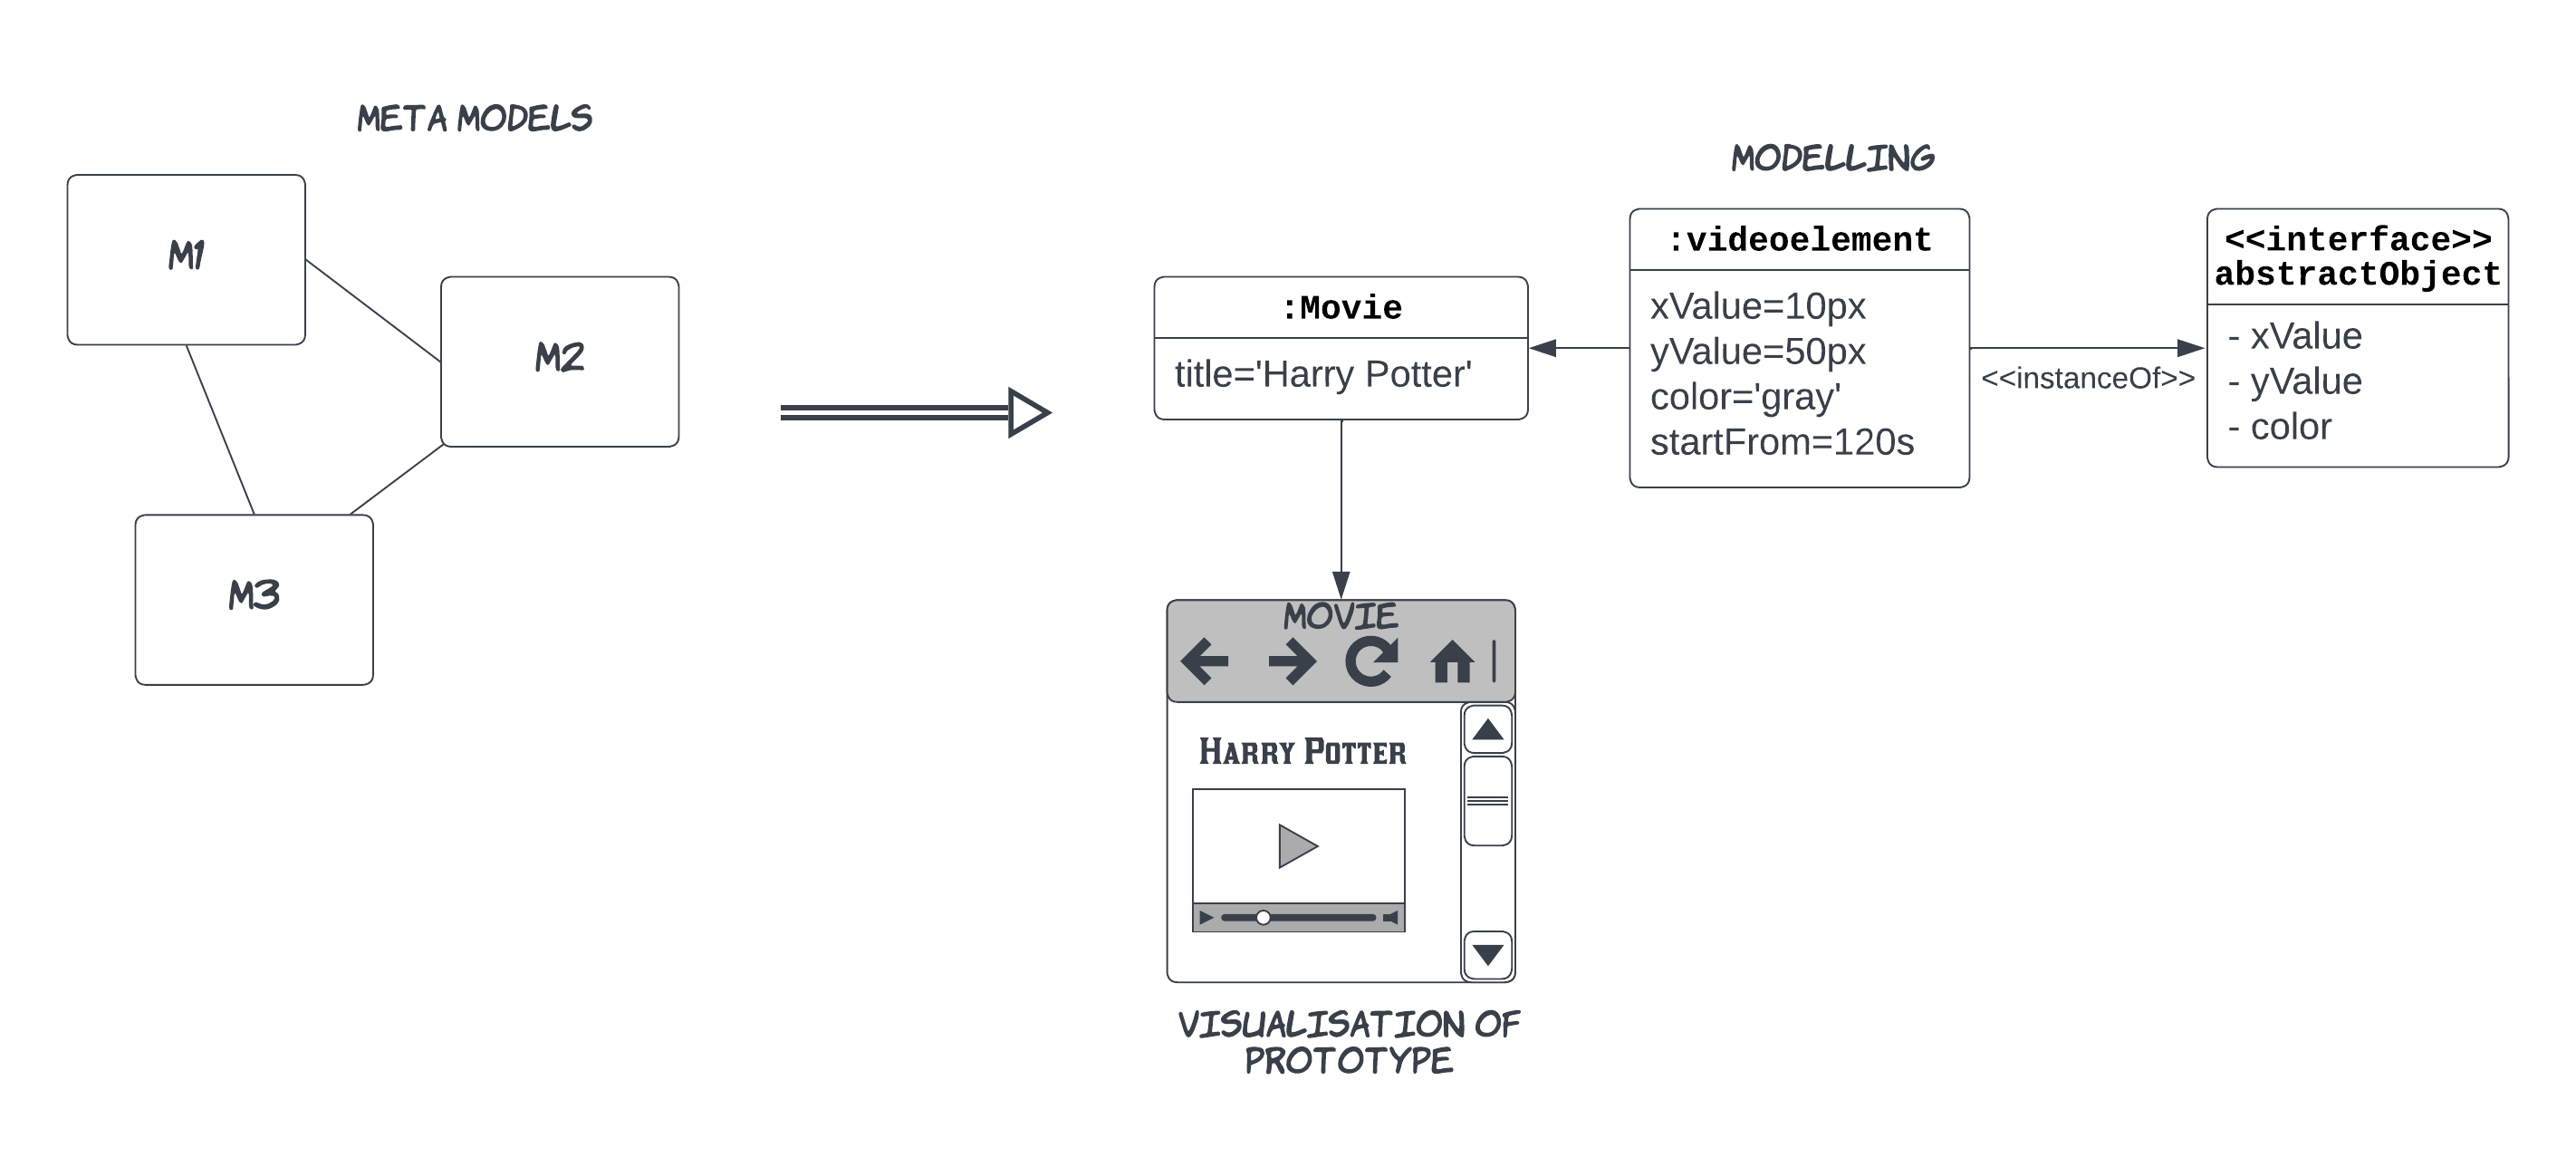
\includegraphics[width=1.05\textwidth]{images/solution-ideas/MetaModel.png}
	\caption{Example Meta Model}
	\label{solutionideas:fig:metamodel}
\end{figure}
\section{Experimenting using A/B Testing}

The product owners continuously investigate new features and product enhancement opportunities by conducting frequent experiments. 
The owners better understand their customers' experiences by creating that feedback loop with users. 
As a result, they can constantly give a practical solution. 
There are various types of experimenting\footnote{A/B Testing: \url{https://www.hotjar.com/conversion-rate-optimization/glossary/ab-testing/}} options available for the product owners.
In our solution, we try to find which of these better fit our requirements and find an approach for conducting experiments with the UI elements. 
The product owner should be able to create various experiments by moving the UI elements and having multiple views for a particular screen. \\ \\
E.g., from our \texttt{Videostreamer app}: As shown in figure \ref{solutionideas:fig:experimentingvariants}, the experiment model can create different variants for the component \texttt{View}: the \texttt{Grid view} (on the left) and the \texttt{List view} (on the right). 
These experiments are conducted on the users by dividing the users into groups and assigning one of the variants to a group. 
This type of setup is called the ``\texttt{Between-group}'' design experiment. 
Then, the users would be given specific tasks as per the \texttt{Task Model}, and the measurements will provide feedback to the \texttt{Experiment Model}. 
The data obtained are analyzed (explained in section \ref{solutionideas:section:dataanalysis}), and finally, we find the best variant for a product's component. 

\begin{figure}[ht]
	\centering
  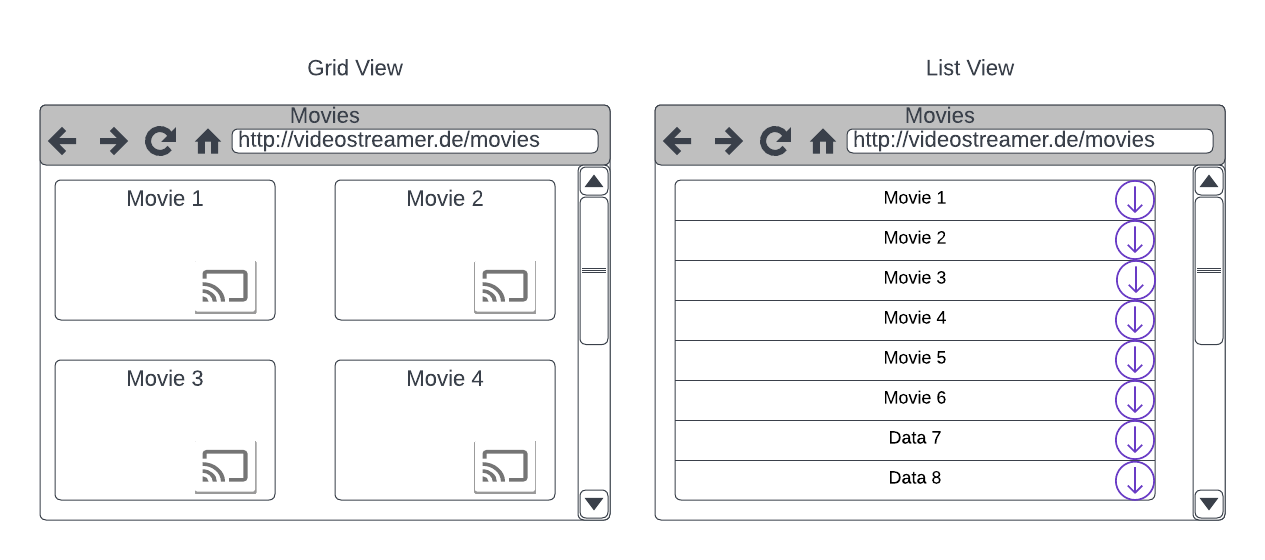
\includegraphics[width=1.0\textwidth]{images/solution-ideas/Experimentvariants.png}
	\caption{Example Experiment variants}
	\label{solutionideas:fig:experimentingvariants}
\end{figure}

\section{Data Analysis}
\label{solutionideas:section:dataanalysis}

In our solution, we focus on model-based and data-driven development. 
As per figure \ref{solutionideas:fig:dddevelopment}, the models provide some data to the data analysis service, receive feedback from it, and tune and improve the model in a continuous and iterative manner. 
For determining the ``Winner'' among the variants of a product's component, we perform data analytics on the feedback data that we receive from the \texttt{Task Model} and the \texttt{Experiment Model}.
We propose to do both \texttt{Quantitative} (presented in section \ref{solutionideas:section:quantitative}) and \texttt{Qualitative} (presented in section \ref{solutionideas:section:qualitative}) analyses of the data.

\begin{figure}[ht]
	\centering
  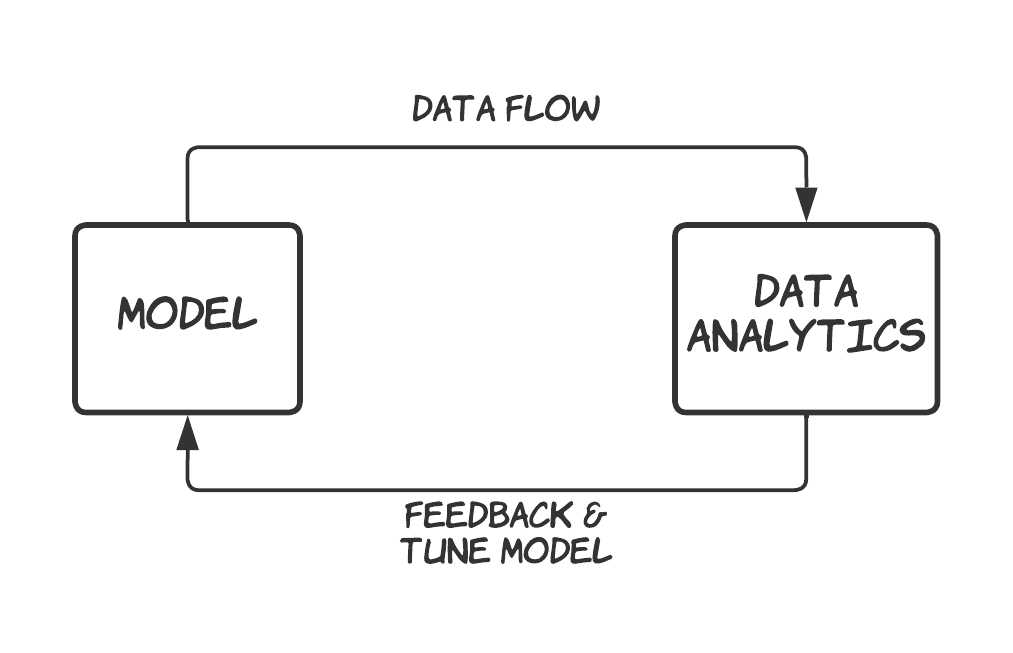
\includegraphics[width=0.5\textwidth]{images/solution-ideas/dd-development.png}
	\caption{Model based Data Driven development}
	\label{solutionideas:fig:dddevelopment}
\end{figure}
\subsection{Quantitative Analysis}
\label{solutionideas:section:quantitative}
Quantitative analysis uses mathematical and statistical methods to determine the behavior of the data and improve performance by tuning the models.
In quantitative research, various descriptive statistics methods like Means, Median, Variances, Standard Deviations, etc., are used. 
We try to find some causal relationships in the data. 

In our solution, from the \texttt{Experiment Model}, we can calculate the measurements on various product components. \\
E.g., from our \texttt{Videostreamer app}: For the View component, the measurements could be ``Watch time'' to measure the duration of time spent by the user on that component's variant, ``Click Rate'' to count the clicks, etc. Then, the experimenting server can calculate the measurements' mean (assume mean is specified in the model by the product owner). 
To validate this data, a significance test can be calculated to determine the probability of the event's occurrence, claim from the mean, and declare the winner variant. \\
Secondly, We also receive the data from the \texttt{Task Model}. 
Its data can be used to calculate the efficiency of the variant. \\
E.g., from our \texttt{Videostreamer app}: If the task is to locate a particular movie, we can calculate the number of clicks and time required for the users to reach the end result (i.e. the movie in the task). \\
This testing type is called ``\texttt{Supervised testing}'' \cite{article:dataanalysis:supervisedtest}.
So, we observe the users, and they know the result (i.e., the movie they need to locate). 
This process gives us more accurate feedback on which variant performs better, and we can then update the product as per our triangle relationship (see fig \ref{solutionideas:fig:triangle}).  

\subsection{Qualitative Analysis}
\label{solutionideas:section:qualitative}
In order to further tune our models, we need to perform qualitative analysis.
Qualitative analysis is used to determine the users' behavior and semantic analysis. 
In qualitative research, the data is usually unstructured as they are from open-ended surveys, interviews, photos, drawings, responses from focus groups, etc. 
Our goal is to turn the unstructured data into a detailed description of the critical aspects of the problem.
In our solution, we propose to perform qualitative analysis of the data by asking some open-ended question to the users.

E.g., from our \texttt{Videostreamer app}: We can ask questions like ``What do you think about the Look and feel of the software application?'', ``Are the items on the page easily locatable?''.
The users' responses can be studied using some tool using the inductive or deductive coding technique. 
If we select the inductive coding approach, we will scrutinize the reactions and those which are similar and group them. 
These groups will be coded into labels, and we will formalize and analyze the categories. 
To understand the process better, see figure \ref{solutionideas:fig:qualitative}. So, we in the end we get a feedback from this process on which of the variants is better for the users. This information can be forwarded to the models for reforming them.
\begin{figure}[ht]
	\centering
  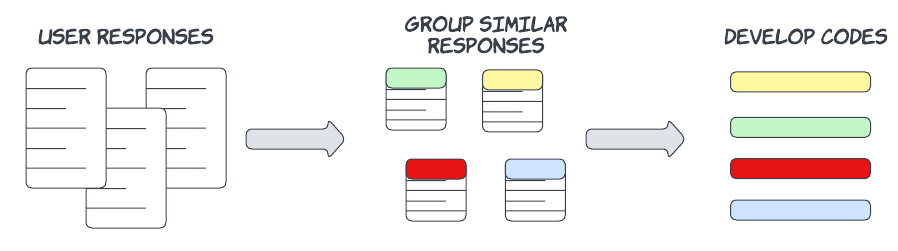
\includegraphics[width=1\textwidth]{images/solution-ideas/qualitative.png}
	\caption{Qualitative analysis using inductive coding}
	\label{solutionideas:fig:qualitative}
\end{figure}